\documentclass{article}
\usepackage[utf8x]{inputenc}
\usepackage[cyr]{aeguill}
\usepackage[francais]{babel}
\usepackage{amsmath,amsfonts,amsthm} % Math packages
\usepackage[pdftex]{graphicx}   
\usepackage{url}
\usepackage{array}
\usepackage{geometry}
\usepackage{float}
\geometry{hmargin=2.5cm,vmargin=1.5cm}
\title{Rapport du projet de représentation des connaissances :\\
De la recherche d'information au Web Sémantique}
\author{Gareau Adrien, Duzan Luc}
\begin{document}
\renewcommand{\labelitemi}{$\bullet$}
\maketitle
\section{Introduction}

Durant ce projet nous avons dû créer un moteur d'indexation et de recherche
d'éléments XML. Notre moteur doit pouvoir retourner une liste de paragraphes
pertinents contenus dans des documents XML. En effet, nous avons une liste de
fichiers XML relatant différents récits sur des balades et notre moteur doit indexer
le contenu de ces fichiers et être capable de faire des recherches sur la collection
de documents.

\section{Indexation des données}

\subsection{Choix de notre structure de données}
La première étape consiste à créer la structure de notre base de données où l’on va
pouvoir stocker les différents termes qui se trouvent dans les fichiers XML. Le
schéma de la figure 1 décrit comment nous avons décidé de créer notre base de données : 

\begin{figure}[h!]
    \centering
    \caption{\label{schéma UML de notre base de donnée} Schéma UML de notre base de
donnée}
    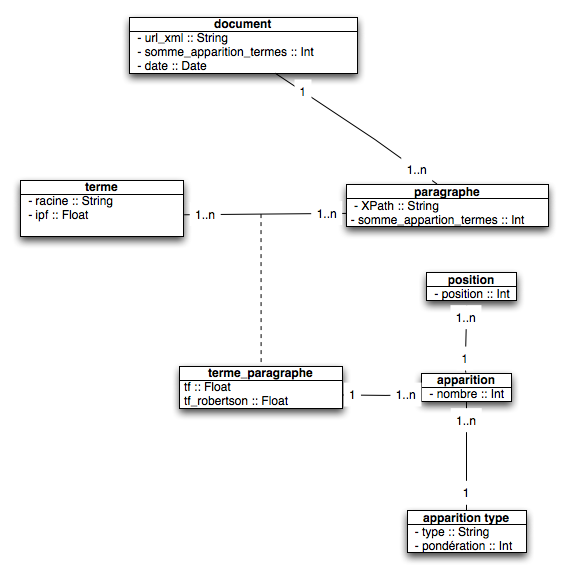
\includegraphics[scale=0.7]{schema_db.png}
\end{figure}

Il est très important de sauvegarder le paragraphe dont le terme provient pour
pouvoir le retourner lors de la phase de recherche. 

Pour chaque terme que l’on va indexer, on ne va stocker que sa racine (voir procédure
d’indexation) ainsi que l’IDF (inverse document frequency) pour ce terme. Pour chaque
terme on sauvegarde les paragraphes dans lesquels il a été trouvé. Pour chaque
association paragraphe-terme, on tient à jour un compteur pour savoir le nombre de
fois que ce terme a été trouvé dans le paragraphe, on enregistre aussi les endroits
où il apparaît dans le paragraphe ou dans des éléments décrivant le paragraphe ( dans
un titre, sous titre ou une description). Cela nous permet aussi de pouvoir mettre
une pondération en fonction de la position du terme.  Dans l’entité document, on
stocke aussi le nombre d’apparitions totales pour un terme dans ce document.
D’ailleurs, la pondération sur le type d’apparition se fait en multipliant les
fréquences des mots :

\begin{itemize}
    \item par 1,5 pour les titres
    \item par 1,5 pour les sous-titres
    \item par 4,0 pour les paragraphes
    \item par 1,25 pour les descriptions
\end{itemize}

De plus, on calcule aussi pour chaque association paragraphe-terme le TF (terme
frequency) ainsi que le TF-robertson (version pondérée du TF). Ainsi pour chaque terme
à la fin de l’indexation on peut aisément calculer le TF-IDF. Nous avons choisi de
stocker ces informations plutôt que de les calculer dynamiquement avant chaque
requête, car nous économisons du temps au niveau des requêtes. En effet l’indexation
ne se fait qu’une seule fois donc il est préférable que cette étape soit plus longue
et ainsi gagner du temps pour les requêtes. 

Concernant la base de données, nous avons décidé d’utiliser PostgreSQL par soucis
pédagogique. Nous voulions nous former sur cet outil très présent dans le monde
industriel.

\subsection{Indexation des données}

Nous nous sommes ensuite penchés sur l’indexation des données. Nous avons tout d’abord
décidé d’utiliser l’API JAXB (Java Architecture for XML Binding )  pour transformer
un fichier XML en objets Java. 

Nous avons ensuite créé les classes correspondantes au schéma de notre base de
données. Le but est de récupérer les informations grâce aux classes générées par
JAXB. 

Le but est de récupérer les informations grâce aux classes générées par JAXB.
L’étape suivante consiste donc  à modifier la classe Balade générée grâce à JAXB. En
effet nous avons créé une méthode qui permet de récupérer tous les paragraphes qui se
trouvent à l’intérieur d’un élément Balade. Nous parcourons le fichier pour récupérer
les paragraphes en sauvegardant leurs positions (Xpath). À ce moment-là, on associe
également au paragraphe ces titres, sous-titres, descriptions correspondantes afin de
pouvoir prendre en compte les mots clefs de ces éléments qui permettent de
contextualiser le paragraphe.  Une fois ces données sauvegardées nous avons défini
une procédure pour formater et indexer les données pour faciliter les recherches
:

\begin{itemize}

    \item Mise en minuscule : afin de rendre la recherche insensible à la case, on
        a mis tout en minuscule. En effet, les êtres humains n’associent pas la case
        des lettres à un sens sémantique et pour eux “Lac” = “lac”

    \item Séparer les mots d’une phrase grâce à des délimiteurs. Il faut séparer
        chaque mot pour obtenir une liste de mots. Nous avons utilisé une expression
        régulière pour trouver tous les signes de ponctuations et d’espace nous
        permettant de délimiter les mots. 

    \item Suppression des stopwords. Grâce à la liste fournie nous pouvons enlever
        tous les mots inutiles lors d’une recherche et donc qui ne nécessitent pas
        d’être stockés dans la base de données. Nous considérons qu’un mot est
        inutile quand il est vide de sens sémantique. Par exemple : “à”, “de” et
        “son”.

    \item Lemmatisation : c’est la réduction en forme canonique de chaque mot. Chaque
        mot va être tronqué en fonction de son champ lexical. Nous avons utilisé le
        lemmatiseur SnowBall. Il permet d’identifier la nature d’un mot et de le
        tronquer de la manière la plus intelligente possible. Cela va permettre de
        rendre nos recherches plus pertinentes, car cet outil va permettre de trouver
        des racines communes avec certains mots alors qu’avec une simple troncature
        cela aurait été impossible. Par exemple une recherche avec le mot clef
        économiser, permettra de trouver des paragraphes contenant les mots économe
        ou encore économie, car ces mots ont tous la même racine.

    \item Suppression des accents :  cela permet de rendre la recherche insensible aux
        accents. En effet, les Français oublient souvent de mettre des accents
        surtout les accents circonflexes.

\end{itemize}


Après avoir formaté ces informations, la partie centrale de l’indexation a été de
parcourir tous les termes afin de calculer le nombre d’apparitions de chacun, en
fonction de leurs positions. On parcourt les différentes balises et on sauvegarde la
position des termes trouvés ainsi que le nombre d’apparitions. Ces informations sont
stockées dans une Map qui va associer les termes au nombre de fois où ils ont été
trouvés.


De plus, nous pondérons les résultats en fonction de la position du terme : si un
terme est trouvé dans le titre il aura un poids plus élevé. Pour un terme trouvé dans
le titre on le pondère de 2,5, 1,5 pour le sous-titre et 1,25 pour la description. En
ce qui concerne les éléments qui sont trouvés dans un paragraphe, ils ont un poids de 4.
En effet, si un terme est trouvé une seule fois dans le titre mais très peu dans le
paragraphe le document ne doit pas se retrouver devant un autre, où certes le terme
n’est pas dans le titre mais beaucoup plus présent dans les paragraphes. C’est
pourquoi nous avons mis un poids assez important pour les apparitions dans les
paragraphes. 

La dernière étape consiste à sauvegarder ces données dans la base de données. Pour
cela, vu le nombre assez conséquent d’insertions à faire nous avons décidé de le
faire à l’aide de “batchs”. Pour éviter d’avoir un débordement de mémoire, la taille
d’un batch ne peut pas accéder 10 000 insertions . L’utilisation de batchs réduit le
temps d’accès à la base et donc le temps d’exécution, qui est d’environ 6-7 minutes.
Juste avant d’insérer les données nous calculons le TF et les IDF. Tout d’abord, nous
utilisons la formule du TF de Robertson vue en cours
: $TF= \frac{\text{fréq}}{0.5 + 1.5 * \frac{\text{longueur doc}}{\text{longueur moyene doc}} + \text{fréq}}$
puis nous utilisons la formule pour calculer l’IDF : $log(\frac{N}{n_i})$, avec N le
nombre de paragraphes et $n_i$ le nombre de paragraphes contenant le terme en question.


\section{Recherche}

\subsection{Récupération des requêtes}

Les différentes requêtes que nous devions exécuter sont stockées dans des fichiers
XML. Nous avons donc à nouveau utilisé JAXB pour les convertir en classes Java. 

\subsection{Formatage des données}

Après avoir stocké les requêtes nous avons utilisé la même procédure que lors de
l’indexation pour formater ces données (mettre tout en minuscule, enlever les
accents, lemmatisation…). 

Les chaines de caractères contenues dans la liste finale seront par la suite désignées par
mot clef, bien qu’en réalité, ils sont lemmatisés (par exemple “amérique” est
lemmatisé en “amer”) nous ne donnerons pas la version lemmatisée.

Nous obtenons donc une liste de mots clefs qui est associée à un poids de un
contrairement au mot clefs déduit de l’interrogation d’une ontologie qui auront un
poids variable.


\subsection{Création de la requête d'interrogation}

Après avoir récupéré les mots clefs associés à la recherche, nous avons créé une
requête qui va récupérer tous les paragraphes qui contiennent au moins un des mots
clefs de la requête. 

De plus nous calculons le TF-IDF pour chaque mot clef et nous stockons ces résultats
dans une “map” de la forme <Token , TF-IDF>, cette “map” correspond alors
conceptuellement à un vecteur. 

Pour finir nous faisons un produit scalaire en la “map” créée avec les mots clefs
contenus dans les paragraphes et la liste de mots clefs récupérée depuis la requête.

\subsection{Sparql}

Comme on peut le voir dans la partie “benchmark”. La technique de recherche se basant
uniquement sur les termes de la requête atteint assez vite ses limites. En effet,
soit on passe à coter des synonymes de ces termes, ou alors on passe à coter de
certains documents qui contiennent des termes plus précis que les termes de la
recherche. Par exemple, une recherche utilisant les termes “Balade en France” passera
à coter d’un paragraphe parlant de “Randonnée à Toulouse” si ce dernier ne contient
ni le mot “France”, ni le mot “balade” alors qu’il parle pourtant bien de balade en
France. Les limites de la recherche par thème uniquement se sentent beaucoup sur des
requêtes telles que :

\begin{itemize}

    \item “balade en Asie”, en effet la plupart des paragraphes concernés ne
        contiennent pas le mot, “Asie” mais le nom d’un pays ou d’une ville d’Asie.

    \item “monuments religieux en Afrique”, même explication que pour l’Asie, de plus
        on parle rarement de monuments, mais plutôt d’un type de monument (église,
        immeuble par exemple)

    \item “animaux Pyrénées”, on ne trouve pas le mot “anima” mais des noms d’animaux
        (chien, chamois etc…).

\end{itemize}


Pour pallier ce problème, nous avons utilisé une ontologie que nous avons interrogée
grâce à SPARQL. Malheureusement l'ontologie n'était pas complète,
surtout au niveau des labels (il n’y avait pas les différentes versions avec ou sans
majuscule, ou encore sans accent). Nous avons effectué une première requête pour
récupérer tous les labels présents dans l’ontolologie. Nous avons ensuite recherché
les labels sans leurs accents et de leurs majuscules sur la requête. Nous avons aussi
enlevé les accents et les majuscules de la requête. Cela nous a permis d’obtenir la
liste des concepts présents dans l’ontologie ainsi que dans la requête. Pour chaque
concept, nous avons effectué les requêtes suivantes afin de rajouter des termes
à notre requête :

\begin{itemize}

    \item chercher les objets qui sont des sous entités (subClassOf) du concept et
        récupérer tous leurs labels

    \item chercher tous les sous lieux de notre entité (si notre entité n’est pas un
        lieu, cela n’a pas de sens mais la requête ne retournera alors rien de toute
        manière)

    \item chercher les lieux à côté de notre entité et récupérer leur label

    \item chercher les synonymes (en fait il s’agit de tous les labels de notre
        entité).

    \item chercher les animaux qui vivent dans notre entité (permet uniquement de
        récupérer lama pour la recherche des balades en Amérique latine, ce qui
        a beaucoup d’importance pour moi, car j’aime beaucoup les lamas).

\end{itemize}

\begin{figure}[H]
    \centering
    \caption{Photographie d'un lamastronaute}
    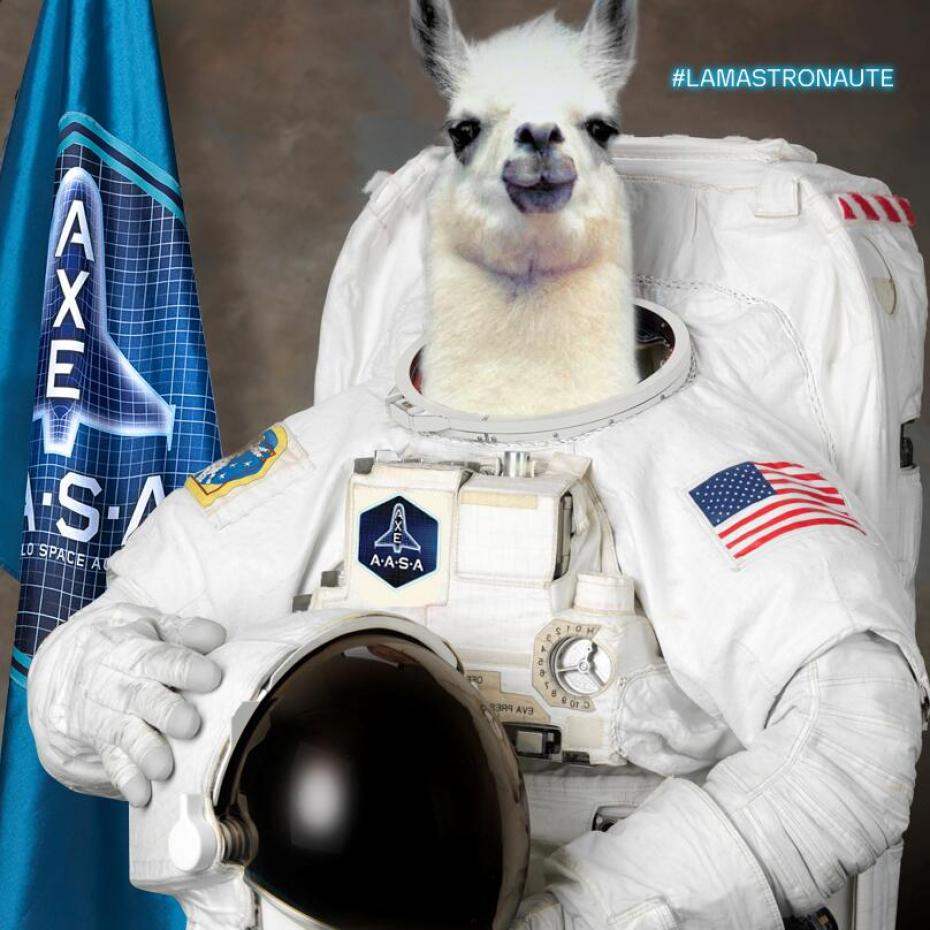
\includegraphics[scale=0.4]{lama.jpg}
\end{figure}

Ces requêtes, nous permettent alors de récupérer de nombreux labels qui sont
alors traités comme les requêtes. C’est-à-dire qu’on leur enlève les accents,
les majuscules, qu’on leur enlève les mots “vide de sens” (stopword), qu’on
découpe le label en mot et qu’on lemmatise ces mots. Ainsi à partir des labels,
on obtient une liste de mots clefs qui sont susceptibles d’être présents dans
notre index inversé. Le problème de cette procédure est qu’elle génère beaucoup
de mots clefs additionnels, il faut alors veiller à limiter “le bruit” amené
par l’ajout de ces mots clefs, qui ont parfois, une fois isolé, une
signification différente par rapport au concept originel présent dans la
requête. Par exemple, la présence du mot “montagne” dans la requête “balade en
montagne en Asie” va permettre de trouver le concept “montagne” dans
l’ontologie qui a pour sous classe (entre autres) “montagne américaine”. Cela
va donner après lemmatisation et séparation des mots le mot clef “amérique”qui
va alors dégrader la qualité de la recherche surtout si ce mot clef n’est pas
pondéré par rapport à Asie (l’exemple ici choisi est le plus catastrophique
mais il est réel). De plus si un mot est associé à un concept dans l’ontologie,
il va alors amener des mots clefs sémantiquement proches de lui dans la
requête. Ce qui risque de diminuer fortement l’influence d’un autre mot qui lui
ne serait pas présent au sein de l’ontologie et qui dans le vecteur final de
recherche serait alors représenté par un seul mot clef.  C’est à ce moment-là
que l’on fait intervenir la pondération des mots clefs du vecteur de recherche
qui était avant systématiquement mis à 1. Maintenant, les mots clefs présents
au sein même de la requête gardent cette pondération de 1. Alors que pour les
mots clefs issus d’un concept présent au sein de la requête se voient assigner
les coefficients de 1,2, s’ils sont issus d’un sous concept, de 1 s’ils sont
issus d’un synonyme ou d’un sous lieu et de 0,3 s’ils sont issus d’un animal
vivant dans le lieu ou d’un lieu à côté. Ensuite, les coefficients des mots
clefs issus d’un même concept sont divisés par leur somme puis multipliés par
1,3 (valeur obtenue empiriquement). Ainsi la représentation totale d’un concept
par ses mots clefs déduientt indirectement est toujours de 1,3.

Malheureusement, l’ontologie n’est pas bien fournie, surtout pour l’Asie où nous
avons rajouté des pays, ainsi que certaines villes. Nous avons également remarqué que la
relation “à côté de” n’était pas exploitée dans l’ontologie. De plus, l’utilisation
qu’on a de l’ontologie amène des fois des mots clefs parasites comme le montre
l’exemple des “montagne en Asie” au-dessus. Une bonne idée aurait été de stocker dans
l’indexe inversé les labels entiers tels qui sont présents dans l’ontologie en plus
des mots clefs lemmatisés, car beaucoup de concept ont des labels sur deux mots
(“Mont Blanc”, “Montagne Amérique”) et que la séparation de ces mots amène souvent
du bruit.

\section{Benchmark}

\subsection{Requête 1 : \og balade au Mont Blanc \fg }

\begin{table}[H]
    \centering
    \caption{Requête 1}
\begin{tabular}{|l|c|c|c|}
    \hline
    Précision à & 5 & 10 & 25 \\
    \hline
    Sans TF.IDF, sans ontologie & 20\% & 20\% &  16\% \\
    \hline
    Avec TF.IDF, sans ontologie & 40\% & 50\% &  48\% \\
    \hline
    Avec TF.IDF, avec ontologie & 40\% & 50\% &  48\% \\
    \hline
\end{tabular}
\end{table}

Sur cette requête, on remarque notamment l'efficacité du tf.idf, en effet beaucoup de
paragraphes contiennent le mot “mont” et peu contiennent le mot blanc. Le tf.idf
permet alors de mettre en avant ceux qui contiennent le mot “blanc” et limite la
pollution des documents qui contiennent le mot “mont”  mais qui n’ont aucun rapport
avec le mot “blanc”. Concernant l’ontologie, elle n’apporte peu de nouveaux mots clefs
sur cette requête et ne permet donc pas d’amélioration.


\subsection{Requête 2 : \og balade montagne Amérique latine \fg }

\begin{table}[H]
    \centering
    \caption{Requête 2}
\begin{tabular}{|l|c|c|c|}
    \hline
    Précision à & 5 & 10 & 25 \\
    \hline
    Sans TF.IDF, sans ontologie & 0\% & 0\% &  0\% \\
    \hline
    Avec TF.IDF, sans ontologie & 0\% & 0\% &  4\% \\
    \hline
    Avec TF.IDF, avec ontologie & 0\% & 0\% &  4\% \\
    \hline
\end{tabular}
\end{table}

Ici le résultat déplorable des recherches sans l’aide de l’ontologie est
compréhensible car quand un document parle d’une balade en Amérique latine, il
n’utilise pas en général le mot “Amérique latine” mais il parle plus souvent d’un
pays spécifique tel que le Pérou. L’utilisation de l’ontologie permet bien de
rajouter une longue liste de pays d’Amérique latine à la requête et le fait que les
résultats sont si mauvais est surprenant. L'analyse des paragraphes trouvés et des
paragraphes attendus montre deux phénomènes expliquant cela :

\begin{itemize}

    \item les paragraphes attendus ne citent pas de pays d’Amérique latine, mais des
        lieux bien plus précis (monument ou lieu naturel) qui ne sont pas dans
        l’ontologie

    \item la liste très longue des pays amènent une grande division de leurs
        coefficients dans le vecteur de requête. Alors que les mots clefs de base
        (“montagne”, “Amérique”, “latine”) ont toujours des coefficients de 1, les
        paragraphes en tête sont ceux qui contiennent et/ou ces mots-là. Or notre
        moteur ne gérant pas “les mots clefs à deux mots”, il remonte des paragraphes
        parlant d’Espagne à cause du mot latin ou de montagnes (qui ne sont pas en
        Amérique latine) à cause de “montagne”.

\end{itemize}

\subsection{Requête 3 : \og monuments Afrique \fg }

\begin{table}[H]
    \centering
    \caption{Requête 3}
\begin{tabular}{|l|c|c|c|}
    \hline
    Précision à & 5 & 10 & 25 \\
    \hline
    Sans TF.IDF, sans ontologie & 20\% & 10\% & 4\% \\
    \hline
    Avec TF.IDF, sans ontologie & 20\% & 10\% & 4\% \\
    \hline
    Avec TF.IDF, avec ontologie & 20\% & 10\% & 4\% \\
    \hline
\end{tabular}
\end{table}

Bien que les résultats ne peuvent conclure à une amélioration de l’utilisation de
l’ontologie, l’analyse des paragraphes sélectionnés montre qu’ils sont aussi
pertinents que ceux attendus.  D'un point de vue personnel, nous trouvons qu’ici la
liste des paragraphes attendus n’est sûrement pas assez complète. L’ontologie a bien
fonctionné, car elle a renvoyé quelques pays d’Afrique (peut-être pas assez tout de
même) et une bonne liste de monument (pyramide, cathédrale etc.)

\subsection{Requête 4 : \og lacs de France \fg }

\begin{table}[H]
    \centering
    \caption{Requête 4}
\begin{tabular}{|l|c|c|c|}
    \hline
    Précision à & 5 & 10 & 25 \\
    \hline
    Sans TF.IDF, sans ontologie & 40\% & 40\% & 28\% \\
    \hline
    Avec TF.IDF, sans ontologie & 60\% & 40\% & 40\% \\
    \hline
    Avec TF.IDF, avec ontologie & 60\% & 40\% & 44\% \\
    \hline
\end{tabular}
\end{table}

Rien de particulier à signaler, hormis que sur cette requête l’ontologie rajoute des
noms de lac français en mots clefs, mais cela ne change rien car leur présence va
souvent de pair avec celle des mots ‘lac’ et ‘France”.

\subsection{Requête 5 : \og liste des monuments religieux visités \fg }

\begin{table}[H]
    \centering
    \caption{Requête 5}
\begin{tabular}{|l|c|c|c|}
    \hline
    Précision à & 5 & 10 & 25 \\
    \hline
    Sans TF.IDF, sans ontologie & 0\% &   20\% &  12\% \\
    \hline
    Avec TF.IDF, sans ontologie & 60\% & 30\% &  12\% \\
    \hline
    Avec TF.IDF, avec ontologie & 60\% & 30\% &  12\% \\
    \hline
\end{tabular}
\end{table}

Bien que l’ontologie est bien fait son travail en rajoutant une longue liste de
monument religieux au sein de la requête, il n’y a pas beaucoup d’amélioration. On
remarque un phénomène similaire à celui de l’Amérique latine, l’isolation des mots
“monuments” et “religieux” retourne des documents qui concernent soit les monuments
soit la religion mais pas les “monuments religieux”.

\subsection{Requête 6 : \og village randonnée montagne Asie \fg }

\begin{table}[H]
    \centering
    \caption{Requête 6}
\begin{tabular}{|l|c|c|c|}
    \hline
    Précision à & 5 & 10 & 25 \\
    \hline
    Sans TF.IDF, sans ontologie & 0\% & 0\% & 0\% \\
    \hline
    Avec TF.IDF, sans ontologie & 0\% & 0\% & 0\% \\
    \hline
    Avec TF.IDF, avec ontologie & 0\% & 0\% & 0\% \\
    \hline
\end{tabular}
\end{table}

Sur ce genre de requête l’utilisation de l’ontologie est plus que nécessaire pour les
mêmes raisons exposées pour la requête concernant l’Amérique latine. L’ontologie était
assez démunie sur ce sujet-là mais nous l’avons comblée. L’analyse des paragraphes
retournés montre qu'ils sont pertinents. Les mauvais résultats sont dûs à la
médiocrité de la sélection des paragraphes attendus, en effet beaucoup concernent la
Bolivie et l’Amérique latine…

\subsection{Requête 7 : \og GR10 rando Pyrénées \fg }

\begin{table}[H]
    \centering
    \caption{Requête 7}
\begin{tabular}{|l|c|c|c|}
    \hline
    Précision à & 5 & 10 & 25 \\
    \hline
    Sans TF.IDF, sans ontologie & 80\% & 80\% & 92\% \\
    \hline
    Avec TF.IDF, sans ontologie & 60\% & 70\% & 64\% \\
    \hline
    Avec TF.IDF, avec ontologie & 100\% & 90\% & 72\% \\
    \hline
\end{tabular}
\end{table}

Rien à signaler, l’ontologie rajoute le mot “grand” pour GR (“grande randonnée”) et
sentier.

\subsection{Requête 8 : \og Animaux Pyrénées \fg }

\begin{table}[H]
    \centering
    \caption{Requête 8}
\begin{tabular}{|l|c|c|c|}
    \hline
    Précision à & 5 & 10 & 25 \\
    \hline
    Sans TF.IDF, sans ontologie & 20\% & 30\% &  12\% \\
    \hline
    Avec TF.IDF, sans ontologie & 40\% & 20\% &  12\% \\
    \hline
    Avec TF.IDF, avec ontologie & 40\% & 20\% &  12\% \\
    \hline
\end{tabular}
\end{table}

Il est étonnant que l’utilisation de l’ontologie n’améliore pas plus les résultats.
L’analyse des paragraphes retournés montre qu’ils sont pertinents. L’ontologie
retourne une grande liste d’animaux. Par contre, elle ne retourne pas de sous lieu
pour les Pyrénées.

\subsection{Requête 9 : \og paysage montagne \fg }

\begin{table}[H]
    \centering
    \caption{Requête 9}
\begin{tabular}{|l|c|c|c|}
    \hline
    Précision à & 5 & 10 & 25 \\
    \hline
    Sans TF.IDF, sans ontologie & 0\% & 0\% & 0\% \\
    \hline
    Avec TF.IDF, sans ontologie & 0\% & 0\% & 8\% \\
    \hline
    Avec TF.IDF, avec ontologie & 0\% & 0\% & 8\% \\
    \hline
\end{tabular}
\end{table}

Ici l’ontologie ajoute plus de bruits qu’autre chose, à cause des sous entités de
montagnes (montagnes d’Asie et montagnes d’Amérique latine) qui amènent alors les mots
clefs “Amérique” et “latine”. L’analyse des paragraphes retournés montre cependant
qu’ils sont pertinents.

\subsection{Requête 10 : \og Glaciers des alpes \fg }

\begin{table}[H]
    \centering
    \caption{Requête 10}
\begin{tabular}{|l|c|c|c|}
    \hline
    Précision à & 5 & 10 & 25 \\
    \hline
    Sans TF.IDF, sans ontologie & 100\% & 100\% & 100\% \\
    \hline
    Avec TF.IDF, sans ontologie & 80\% & 90\% & 96\% \\
    \hline
    Avec TF.IDF, avec ontologie & 100\% & 90\% & 92\% \\
    \hline
\end{tabular}
\end{table}

Rien à signaler, si ce n’est la légère chute du à l’utilisation de l’ontologie
sûrement à cause de l’ajout du mot lac qui génère du “bruit”.

\subsection{Requête 11 : \og plongée sous marine \fg }

\begin{table}[H]
    \centering
    \caption{Requête 11}
\begin{tabular}{|l|c|c|c|}
    \hline
    Précision à & 5 & 10 & 25 \\
    \hline
    Sans TF.IDF, sans ontologie & 40\% & 30\% & 12\% \\
    \hline
    Avec TF.IDF, sans ontologie & 40\% & 20\% & 16\% \\
    \hline
    Avec TF.IDF, avec ontologie & 40\% & 20\% & 16\% \\
    \hline
\end{tabular}
\end{table}

Rien à signaler, l’ontologie n’amène pas de nouveaux mots clefs.

\subsection{Moyenne}

\begin{table}[H]
    \centering
    \caption{Moyenne}
\begin{tabular}{|l|c|c|c|}
    \hline
    Précision à & 5 & 10 & 25 \\
    \hline
    Sans TF.IDF, sans ontologie & 29\% &   30\% &  25\% \\
    \hline
    Avec TF.IDF, sans ontologie & 36\% &   30\% &  28\% \\
    \hline
    Avec TF.IDF, avec ontologie & 42\% &   32\% &  29\% \\
    \hline
\end{tabular}
\end{table}


\section{Conclusion}

En conclusion , malgré les améliorations obtenues grâce à l’utilisation de SPARQL
dans notre projet nous obtenons des résultats qui pourraient être améliorés. En
effet, en regardant l’ontologie on remarque que tous les éléments n’ont pas de
labels. Il faudrait donc retravailler l’ontologie pour obtenir de meilleurs
résultats. Il faudrait également revoir les index utilisaient pour prendre en
considération dés l'indexation la sémantique de l’ontologie. Ce n’est pas seulement
le code qui va nous donner de bons résultats mais aussi l’ontologie sur laquelle nous
faisons nos requêtes. 

\end{document}


